\subsection{Initial Testing}
Upon beginning the experiment, students were first instructed to test the provided circuit to ensure that it is working.  While powered, the pin labeled~$V_\text{CC}$ was to measure~\SI{5}{\volt}, the LEDs were to measure~\SI{3.2}{\volt}, and pin 3 of the DAC was to measure around~\SI{-14}{\volt}.  These values were recorded and are tabulated in Table~\ref{tab:initTest}.
%
\begin{table}[H]
	\centering
	\begin{tabular}{|c|c|c|c|}
	\hline
	\tbf{Location} & \tbf{Expected Value (\si{\volt})} &
		\tbf{Measured Value (\si{\volt})} & \tbf{Error (\si{\percent})} \\ \hline
	$V_\text{CC}$  & 5.000 & 5.120 & 2.4  \\ \hline
	$V_\text{LED}$ & 3.200 & 3.158 & -1.3 \\ \hline
	$V_\text{EE}$  &-14.00 &-14.75 & 5.4 \\ \hline
\end{tabular}

	\parbox{.6\textwidth}{
	\caption[Measured Initial Values]{List of values recorded during the initial testing phases.  The voltages were within reasonable limits, allowing the student to safely assume that the board was operating correctly.}
	\label{tab:initTest}}
\end{table}
%
Next, the student shorted the input terminal to ground, ensuring that all eight LEDs from the ADC were lit.  The voltage at the DAC's output was measured at~\SI{-1.4}{\milli\volt}~--- reasonably close to the expected value of zero volts, implying proper operation.

\subsection{ADC/DAC DC Test}
The input short to ground was removed in place of the in-lab DC voltage supply.  With the current limited to~\SI{0.2}{\ampere}, the voltage was varied from zero to five volts in increments of one, measuring the output voltage at each step and tabulating all recorded voltages in Table~\ref{tab:dcSweep}.
%
\begin{table}[H]
	\centering
	\begin{tabular}{|c|c|c|c|}
	\hline
	\tbf{Input (\si{\volt})} &
		\tbf{Expected Output (\si{\volt})} &
		\tbf{Measured Output (\si{\volt})} & \tbf{Error (\si{\percent})} \\ \hline
	0  & 0  & 0      & 0 \\ \hline
	1  & -1 & -0.957 & -4.26 \\ \hline
	2  & -2 & -1.901 & -4.95 \\ \hline
	3  & -3 & -2.865 & -4.50 \\ \hline
	4  & -4 & -3.742 & -6.45 \\ \hline
	5  & -5 & -4.300 & -14.0 \\ \hline
\end{tabular}

	\parbox{.6\textwidth}{
	\caption[DC Sweep Results]{Data recorded from a DC sweep performed with all eight DIP switches closed.}
	\label{tab:dcSweep}}
\end{table}
%
As is clearly visible in the recorded values, the output tended to be slightly higher than the expected output (note that since the output was expected to be negative as previously stated, the error is still calculated to be negative as well).  Since all eight of the switches between the ADC and DAC were closed for this sweep, the output voltages were close to their theoretical values.  Additionally, theoretical values were simply the negative value of the input and were not directly calculated.  This is a result of the known-working ADC being used to create a valid series of bits for the DAC's input.

Next, the input voltage was locked at one volt and a series of DIP switches between the ADC and DAC were opened so that students could observe the effects of a changing digital input.  The switches associated with bits~0,~1,~3,~5, and~7 were opened one at a time, while recording the output voltage corresponding to each configuration.  Table~\ref{tab:1vDIPs} contains the measured voltages for each state.
%
\begin{table}[H]
	\centering
	\begin{tabular}{|c|c|}
	\hline
	\tbf{Open Bit} & \tbf{Meaured Output (\si{\milli\volt})} \\ \hline
	None & -957  \\ \hline
	0    & -970  \\ \hline
	1    & -954  \\ \hline
	3    & -1106 \\ \hline
	5    & -953  \\ \hline
	7    & -3390 \\ \hline
\end{tabular}

	\parbox{.6\textwidth}{
	\caption[\SI{1}{\volt}DC DIP Switches]{Measured output for various DIP switch configurations with a~\SI{1}{\volt} input.}
	\label{tab:1vDIPs}}
\end{table}
%
For a one volt input, the associated ADC output is~\texttt{0011 0010}.  The DAC is logic-one based but the LEDs are logic-zero activated, so each bit passes through an inverter before entering the DAC (after leaving the DIP switches).  This means that opening a switch will only have an effect on bits that are zero as they pass through the switches~(i.e. bits~0,~2,~3,~6, and~7).  Note the drastic effect that bit seven has on the output voltage, as it is the most-significant bit.

The DIP switch test was repeated with an input of five volts.  The results of this test are tabulated in Table~\ref{tab:5vDIPs}.
%
\begin{table}[H]
	\centering
	\begin{tabular}{|c|c|}
	\hline
	\tbf{Open Bit} & \tbf{Meaured Output (\si{\volt})} \\ \hline
	None &  4.313 \\ \hline
	0    &  4.313 \\ \hline
	1    &  4.314 \\ \hline
	3    &  4.471 \\ \hline
	5    &  4.311 \\ \hline
	7    &  4.313 \\ \hline
\end{tabular}
\\
	\parbox{.6\textwidth}{
	\caption[\SI{5}{\volt}DC DIP Switches]{Output measured for several DIP switch states for a~\SI{5}{\volt} input to the ADC.}
	\label{tab:5vDIPs}}
\end{table}
%
The ADC output associated with a~\SI{5}{\volt} input in this case was~\texttt{1110 0010}; as with the~\SI{1}{\volt} test, only bits of value zero (as output by the ADC) are effected by a change in DIP switch.  In this case, only bits zero and three have the potential to change the output voltage of the DAC.  While a change in output is visible for bit three, there is a negligible change due to bit zero, as it is the least significant.

\subsection{ADC/DAC AC Test}
Once the properties of a DAC had been examined for a static input, a sinusoidal input was used in place of the DC source to test the system's performance under varying conditions.  With the in-lab function generator providing a~\SI{400}{\hertz} signal ranging from zero to~\SI{4}{\volt} as shown in the upper signal~(A1) of Figure~\ref{fig:pt4a}, the DAC produced the lower waveform~(A2).
%
\begin{figure}[H]
	\centering
	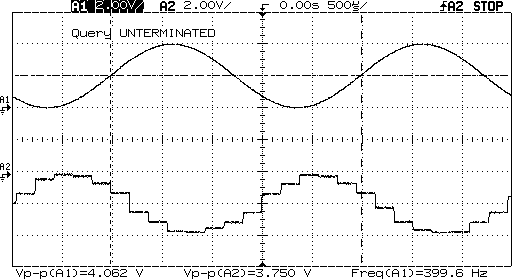
\includegraphics[width=.6\textwidth]{img/shot/pt4ashot.png}
	\parbox{.6\textwidth}{
	\caption[\SI{400}{\hertz} Sine Wave --- All Closed]{DAC output for a~\SI{400}{\hertz} sine wave input.  Note that the output does resemble the input (albeit of the opposite polarity) despite its quantized nature.}
	\label{fig:pt4a}}
\end{figure}
%
As can be seen in the above image, the output waveform greatly resembles the input waveform.  While the output is a negative representation of the input, this is expected behavior.

Just as the DC system was tested for various DIP switch configurations, the AC system was tested.  For each of bits zero, five, and seven, a single switch was opened, and the output recaptured (displayed in Figure~\ref{fig:pt4b}.
%
\begin{figure}[H]
	\centering
	\subfloat[Bit zero open] {\label{subfig:pt4b_bit0}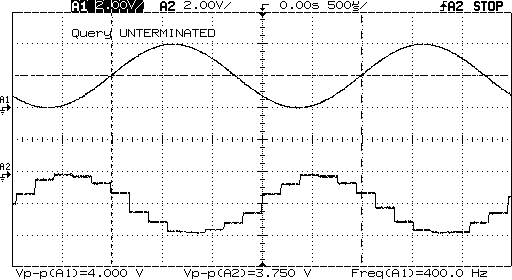
\includegraphics[width=.3\textwidth]{img/shot/pt4b_bit0.png}}
	\quad
	\subfloat[Bit five open] {\label{subfig:pt4b_bit5}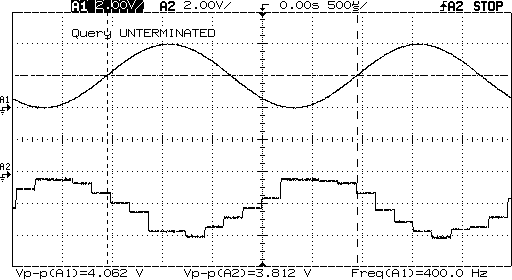
\includegraphics[width=.3\textwidth]{img/shot/pt4b_bit5.png}}
	\quad
	\subfloat[Bit seven open]{\label{subfig:pt4b_bit7}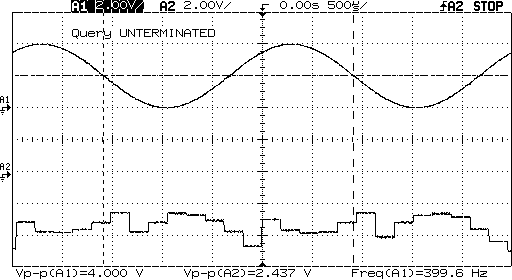
\includegraphics[width=.3\textwidth]{img/shot/pt4b_bit7.png}}

	\parbox{.8\textwidth}{
	\caption[\SI{400}{\hertz} Sine Wave --- DIP Switches]{Results of varying the open DIP switch for a~\SI{400}{\hertz} sinusoidal input.  Note that, where bit five is opened in~\subref{subfig:pt4b_bit5}, the upper portions of the sinusoid are not represented.  Similarly,~\subref{subfig:pt4b_bit7} shows a nearly complete loss of a recognizable signal when bit seven is opened.}
	\label{fig:pt4b}}
\end{figure}
%
\emph{Because the changing shape of the output is the intended focus of this test, screenshots for each configuration are shown next to each other for easy comparison.  Full-sized versions are available in the Appendix, and specific measurements from each are aggregated in Table~\ref{tab:pt4b}.}
%
\begin{table}[H]
	\centering
	\begin{tabular}{|c|c|}
	\hline
	\tbf{Open Bit} & \tbf{Meaured Voltage (\si{\volt}, P-P)}\\ \hline
	None & 3.750  \\ \hline
	0    & 3.750  \\ \hline
	5    & 3.812  \\ \hline
	7    & 2.437  \\ \hline
\end{tabular}

	\parbox{.6\textwidth}{
	\caption[\SI{400}{\hertz} Sine Wave --- DIP Switches]{Measured output of a varying state of DIP switch positions for a~\SI{400}{\hertz} sinusoidal input.}
	\label{tab:pt4b}}
\end{table}
%
While in the DC case the output voltage distorted, in the AC case the effects are exaggerated.  The frequency of the output appears to remain roughly constant (this was difficult to measure due to the oscilloscope limitations), but the peak-to-peak voltage accuracy degrades as more-significant bits are opened via DIP switch.  This, coupled with the loss of accurate value representation, produces an increasingly distorted signal that becomes almost unrecognizable in the case of the most-significant bit's opening.

\subsection{Square Wave Input}
The function generator was now tuned to create a square wave with the same amplitude and frequency as the previously-used sine wave.  The DAC output for an input of the aforementioned square wave can be seen in the lower signal of Figure~\ref{fig:pt5a}, while the input is shown in the upper signal.
%
\begin{figure}[H]
	\centering
	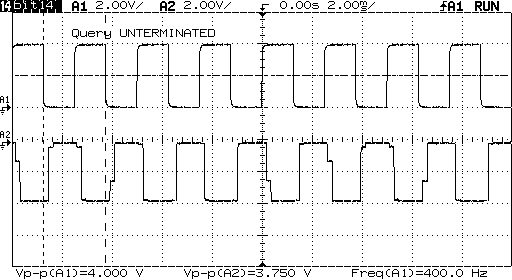
\includegraphics[width=.6\textwidth]{img/shot/pt5a_noopen.png}
	\parbox{.6\textwidth}{
	\caption[\SI{400}{\hertz} Square Wave --- All Closed]{DAC input and output signal for a~\SI{400}{\hertz} square wave.  The input is shown above with the output below.  Note that, like the sinusoid and DC signals previously, the output is of opposite polarity to the input.}
	\label{fig:pt5a}}
\end{figure}
%
A square wave --- just as a sinusoidal wave --- produces an output that is similar in shape and magnitude to the input, but has a reversed polarity.

In order to confirm the previously found effects of opened DIP switches on the output waveform, a similar test was again repeated for a square wave input.  The least-significant and most-significant bits were opened separately, producing the outputs shown in Figure~\ref{fig:pt5b}.
%
\begin{figure}[H]
	\centering
	\subfloat[Bit zero open] {\label{subfig:pt5b_bit0}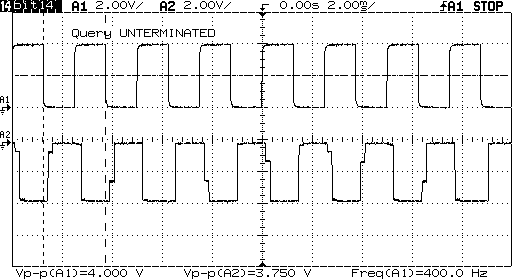
\includegraphics[width=.45\textwidth]{img/shot/pt5b_bit0.png}}
	\quad
	\subfloat[Bit seven open]{\label{subfig:pt5b_bit7}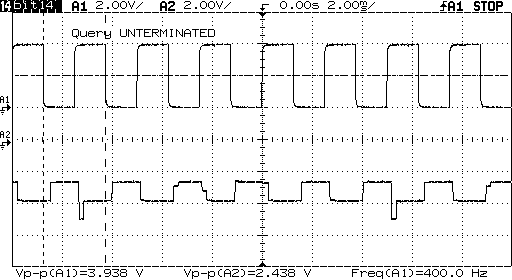
\includegraphics[width=.45\textwidth]{img/shot/pt5b_bit7.png}}

	\parbox{.8\textwidth}{
	\caption[\SI{400}{\hertz} Square Wave --- DIP Switches]{Results of varying the open DIP for a~\SI{400}{\hertz} square wave input.  In an identical result to the sinusoidal case, the output signal's amplitude degrades as a more significant bit is opened.  Opening bit zero has little effect, but opening the most significant bit causes the output to barely resemble the input.}
	\label{fig:pt5b}}
\end{figure}
%
\emph{Because the changing shape of the output is the intended focus of this test, screenshots for each configuration are shown next to each other for easy comparison.  Full-sized versions are available in the Appendix, and specific measurements from each are aggregated in Table~\ref{tab:pt5b}.}
%
\begin{table}[H]
	\centering
	\begin{tabular}{|c|c|}
	\hline
	\tbf{Open Bit} & \tbf{Meaured Voltage (\si{\volt}, P-P)}\\ \hline
	None & 3.750  \\ \hline
	0    & 3.750  \\ \hline
	7    & 2.438  \\ \hline
\end{tabular}

	\parbox{.6\textwidth}{
	\caption[\SI{400}{\hertz} Square Wave --- DIP Switches]{Measured output of a varying state of DIP switch positions for a~\SI{400}{\hertz} square wave input.}
	\label{tab:pt5b}}
\end{table}
%
Similar to the case of the sinusoidal wave, the peak-to-peak voltage of the output signal decreases for an increasing significance of opened bit.  For the most significant bit, a loss of resolution and decreased amplitude combine to produce a nearly unidentifiable output signal, shown in Figure~\ref{subfig:pt5b_bit7}.

\subsection{Word Time}
For each output voltage generated by the DAC, it must read the value of all eight bits and convert this into an analog voltage.  This takes a finite amount of time known as the~``word time,'' from the calling the smallest amount of data needed for a single instruction a~``word.''  It can be measured by passing any time-varying signal into the ADC-DAC system and using the oscilloscope to measure the time between output voltage changes.  In this case, the~\SI{400}{\hertz} sine wave from the AC test was used.  An oscilloscope screenshot of such a measurement is shown in Figure~\ref{fig:pt6a}.
%
\begin{figure}[H]
	\centering
	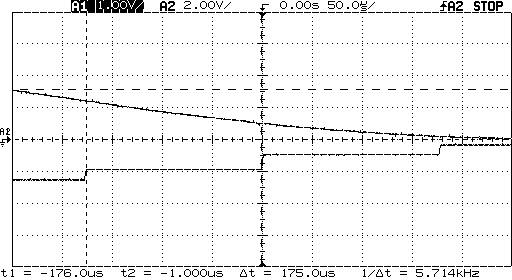
\includegraphics[width=.6\textwidth]{img/shot/pt6a_wordtime.png}
	\parbox{.6\textwidth}{
	\caption[Word Time Measurement --- \SI{400}{\hertz} Sinusoid]{Oscilloscope screenshot showing measurement of the word time for the DAC circuit, using a~\SI{400}{\hertz} sinusoid as the input.}
	\label{fig:pt6a}}
\end{figure}
%
The word time for this system as measured by the oscilloscope is just~\SI{175}{\micro\second}.  It is roughly~70x larger than the period of the ADC's clock, which was measured at~\SI{2.697}{\micro\second}.  Logically, this makes sense, as the system requires roughly eight clock pulses per bit to generate an output voltage~(64 total in this case), and another four to prepare for the next measurement, hence the provided Equation~\eqref{eq:wordtime}.
%
\begin{equation}
	t_\text{word} = 70 t_\text{clk} = 70 \frac{1}{f_\text{clk}} \label{eq:wordtime}
\end{equation}
%
Students next adjusted the input sinusoid's voltage to be~\SI{800}{\hertz} in order to test for the word time's dependency on the input.  The results of such a change are shown in Figure~\ref{fig:pt6b}.
%
\begin{figure}[H]
	\centering
	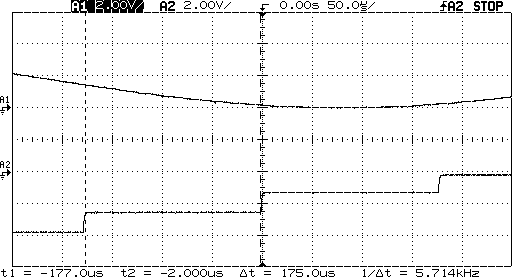
\includegraphics[width=.6\textwidth]{img/shot/pt6b_wordtime.png}
	\parbox{.6\textwidth}{
	\caption[Word Time Measurement --- \SI{800}{\hertz} Sinusoid]{Oscilloscope screenshot showing the measurement of the system's word time for an~\SI{800}{\hertz} input signal.  Note that this time is identical to the time measured in Figure~\ref{fig:pt6a}.}
	\label{fig:pt6b}}
\end{figure}
%
As is expected, the word time was found to be identical to the slower sinusoid, at~\SI{175}{\micro\second}.  This proves that the word time of the system is dependent only on the clock frequency of the system, and not on the input.  If the system's conversion rate was dependent on its input frequency, this particular circuit would be limited to a very small number of possible applications.


